\documentclass[aspectratio=169,10pt]{beamer}

\usetheme{Boadilla}
\usefonttheme{professionalfonts}
\setbeamertemplate{navigation symbols}{}
\setbeamertemplate{footline}[frame number]

\usepackage{graphicx}
\usepackage{booktabs}
\usepackage{array}
\usepackage{xcolor}
\usepackage{tikz}
\usetikzlibrary{arrows.meta,positioning}

\graphicspath{{img/}{img/visuals/}}

\definecolor{motblue}{HTML}{1F4E79}
\definecolor{motgreen}{HTML}{28724F}
\definecolor{motgray}{HTML}{4A4A4A}
\definecolor{motlight}{HTML}{EDF3F7}

\setbeamercolor{title}{fg=motblue}
\setbeamercolor{frametitle}{fg=motblue}
\setbeamercolor{structure}{fg=motblue}
\setbeamercolor{block title}{fg=white,bg=motblue}
\setbeamercolor{block body}{fg=black,bg=motlight}

\newcommand{\tightitem}{\setlength{\itemsep}{0.35em}}
\newcommand{\method}[1]{\texttt{\small #1}}
\newcommand{\mainmsg}[1]{\vspace{0.4em}{\color{motgreen}\small\textbf{#1}}}
\newcommand{\twovisualslide}[6]{
  \begin{frame}{#1}
    \centering
    \begin{columns}[T,onlytextwidth]
      \column{0.49\textwidth}
      \centering
      \textbf{\small #2}\\[0.25em]
      \includegraphics[width=\linewidth]{#3}
      \column{0.49\textwidth}
      \centering
      \textbf{\small #4}\\[0.25em]
      \includegraphics[width=\linewidth]{#5}
    \end{columns}
    \vfill
    \begin{minipage}{0.94\linewidth}
      \centering
      {\color{motgreen}\small\textbf{#6}}
    \end{minipage}
  \end{frame}
}
\newcommand{\singlevisualslide}[4]{
  \begin{frame}{#1}
    \centering
    \textbf{\small #2}\\[0.25em]
    \includegraphics[width=0.86\linewidth,height=0.70\textheight,keepaspectratio]{#3}
    \vfill
    \begin{minipage}{0.94\linewidth}
      \centering
      {\color{motgreen}\small\textbf{#4}}
    \end{minipage}
  \end{frame}
}

\title[VisDrone MOT]{Detection and Tracking in VisDrone2019-MOT}
\subtitle{Detector-limited failures, camera motion, and small-object tradeoffs}
\author{Computer Vision MOT Project}
\institute{VisDrone2019-MOT validation split}
\date{\today}

\begin{document}

\begin{frame}
  \titlepage
  \vspace{-1em}
  \begin{center}
    \small Modular detection + tracking experiments with MOT-format evaluation.
  \end{center}
\end{frame}
% Speaker note: Introduce the project as a targeted MOT study, not just a leaderboard run.

\begin{frame}{Problem and Dataset}
  \begin{columns}[T,onlytextwidth]
    \column{0.52\textwidth}
    \textbf{Drone MOT challenges}
    \begin{itemize}
      \tightitem
      \item Small cars and pedestrians at low pixel area
      \item Occlusion and dense road/intersection scenes
      \item Moving camera breaks image-space motion assumptions
      \item Blur and viewpoint changes reduce detector recall
    \end{itemize}

    \column{0.42\textwidth}
    \textbf{Evaluation scope}
    \begin{itemize}
      \tightitem
      \item Dataset: VisDrone2019-MOT-val
      \item Classes: pedestrian and car
      \item MOT metrics: MOTA, IDF1, IDS, FPS
      \item Detection diagnosis: precision, recall, AP50
    \end{itemize}
  \end{columns}

  \mainmsg{Main question: are failures caused by missed detections, bad associations, false positives, or speed tradeoffs?}
\end{frame}
% Speaker note: Set up the diagnostic framing used later in the deck.

\begin{frame}{Modular Pipeline}
  \centering
  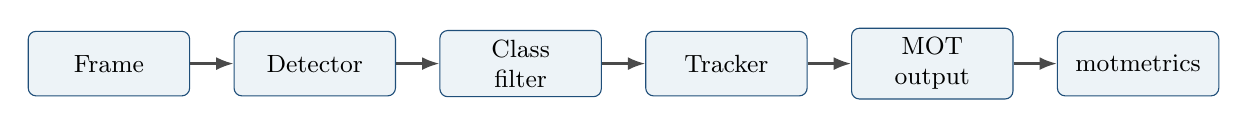
\begin{tikzpicture}[
    node distance=0.55cm,
    pipebox/.style={draw=motblue, rounded corners=1mm, fill=motlight, minimum width=2.05cm, minimum height=0.82cm, align=center, font=\small},
    arrow/.style={-{Latex[length=2.2mm]}, thick, draw=motgray}
  ]
    \node[pipebox] (frame) {Frame};
    \node[pipebox, right=of frame] (det) {Detector};
    \node[pipebox, right=of det] (filter) {Class\\filter};
    \node[pipebox, right=of filter] (track) {Tracker};
    \node[pipebox, right=of track] (mot) {MOT\\output};
    \node[pipebox, right=of mot] (eval) {motmetrics};
    \draw[arrow] (frame) -- (det);
    \draw[arrow] (det) -- (filter);
    \draw[arrow] (filter) -- (track);
    \draw[arrow] (track) -- (mot);
    \draw[arrow] (mot) -- (eval);
  \end{tikzpicture}

  \vspace{1em}
  \begin{columns}[T,onlytextwidth]
    \column{0.48\textwidth}
    \textbf{Design choice}
    \begin{itemize}
      \tightitem
      \item Detector and tracker are decoupled
      \item \texttt{det/} detections are ignored
      \item Outputs are saved in MOT format
    \end{itemize}

    \column{0.48\textwidth}
    \textbf{Why this matters}
    \begin{itemize}
      \tightitem
      \item Detection-only diagnosis before tracking
      \item Tracker ablations without changing detector
      \item Per-sequence failure analysis
    \end{itemize}
  \end{columns}
\end{frame}
% Speaker note: Emphasize that the framework supports interpretable ablations.

\begin{frame}{Methods Compared}
  \centering
  \small
  \begin{tabular}{@{}p{0.12\linewidth}p{0.28\linewidth}p{0.45\linewidth}@{}}
    \toprule
    Group & Method & Role \\
    \midrule
    M1 & YOLOv11 + SORT & Geometric baseline: Kalman prediction + IoU assignment \\
    M2 & YOLO26 + ByteTrack & Fast confidence-aware baseline with low-confidence recovery \\
    M3 & RT-DETR + BoT-SORT & Accuracy-oriented detector with appearance cues and GMC \\
    M4 & SAHI / upscaling variants & Small-object strategies for low-resolution targets \\
    \bottomrule
  \end{tabular}

  \vspace{0.9em}
  \mainmsg{The experiments are compact: each method probes a specific failure mode instead of expanding a blind grid.}
\end{frame}
% Speaker note: Connect each method family to the project statement's innovation requirement.

\begin{frame}{YOLO26 vs RT-DETR}
  \centering
  \small
  \begin{tabular}{@{}p{0.23\linewidth}p{0.31\linewidth}p{0.31\linewidth}@{}}
    \toprule
    & YOLO26 & RT-DETR \\
    \midrule
    Detector type & One-stage dense detector & Transformer detector \\
    Prediction style & Local, grid/anchor-like dense predictions & Query-based global reasoning \\
    Strength & High FPS; strong baseline precision & Better context for crowded aerial scenes \\
    Weakness & Small objects can be missed & Slower; threshold sensitive \\
    MOT implication & Good speed and usable MOTA & Higher recall can help, but FP control is critical \\
    \bottomrule
  \end{tabular}

  \vspace{0.9em}
  \mainmsg{RT-DETR is attractive for aerial scenes because global context can recover small or ambiguous cars, but it must be calibrated for tracking.}
\end{frame}
% Speaker note: Keep architecture explanation compact and practical.

\begin{frame}{Tracking: Geometry vs Appearance}
  \centering
  \small
  \begin{tabular}{@{}p{0.20\linewidth}p{0.36\linewidth}p{0.30\linewidth}@{}}
    \toprule
    Tracker & Association signal & Failure pressure \\
    \midrule
    SORT & Kalman motion + IoU & Camera motion, occlusion, similar nearby targets \\
    ByteTrack & High/low confidence detections + IoU & Better recall use, still mostly geometric \\
    BoT-SORT & Motion + IoU + appearance/ReID + GMC & More robust IDs, slower and detector-dependent \\
    \bottomrule
  \end{tabular}

  \vspace{0.9em}
  \begin{block}{Interpretation}
    Pure geometry is fragile when the camera moves or objects overlap. Appearance embeddings and global motion compensation add association cues that reduce identity fragmentation.
  \end{block}
\end{frame}
% Speaker note: This justifies appearance embeddings versus purely geometric tracking.

\begin{frame}{Baseline Run: First Diagnosis}
  \centering
  \footnotesize
  \renewcommand{\arraystretch}{1.12}
  \begin{tabular*}{\textwidth}{@{\extracolsep{\fill}}lrrrrrr@{}}
    \toprule
    Method & MOTA & IDF1 & IDS & FP & FN & FPS \\
    \midrule
    M1 YOLOv11 + SORT & 0.137 & 0.336 & 515 & 11.9k & 43.0k & 40.3 \\
    M2 YOLO26 + ByteTrack & 0.169 & 0.341 & 384 & 8.8k & 44.2k & 56.5 \\
    M3 RT-DETR + BoT-SORT & \textbf{0.214} & \textbf{0.436} & \textbf{102} & 8.8k & 41.5k & 4.6 \\
    M4 SAHI + ByteTrack & 0.006 & 0.377 & 668 & 29.8k & \textbf{33.4k} & 3.9 \\
    \bottomrule
  \end{tabular*}

  \vspace{0.55em}
  \begin{columns}[T,onlytextwidth]
    \column{0.48\textwidth}
    \textbf{Initial read}
    \begin{itemize}
      \tightitem
      \item M2 was the fast practical baseline.
      \item M3 reduced FN and IDS, showing useful association.
    \end{itemize}
    \column{0.48\textwidth}
    \textbf{Problem}
    \begin{itemize}
      \tightitem
      \item RT-DETR was threshold-sensitive.
      \item SAHI recall gains produced too many false tracks.
    \end{itemize}
  \end{columns}

  \mainmsg{Failure mode: high recall can hurt MOTA if false positives explode.}
\end{frame}
% Speaker note: These rows come from the early full summary used by Analysis-2.

\twovisualslide
  {Crossroad Failure: YOLO26 vs Ground Truth}
  {YOLO26 baseline}
  {crossroad_gt_vs_yolo26_frame058_yolo26.jpg}
  {Ground truth}
  {crossroad_gt_vs_yolo26_frame058_gt.jpg}
  {Many small cars are never detected, so the tracker cannot recover them.}
% Speaker note: uav0000305_00000_v frame 58; YOLO26 has 3 tracks versus 26 GT boxes.

\twovisualslide
  {Crossroad Improvement: RT-DETR + BoT-SORT + GMC}
  {RT-DETR conf055 + GMC}
  {crossroad_gt_vs_rtdetr_frame058_rtdetr055.jpg}
  {Ground truth}
  {crossroad_gt_vs_rtdetr_frame058_gt.jpg}
  {RT-DETR improves car coverage, but many tiny objects remain missed.}
% Speaker note: uav0000305_00000_v frame 58; final method has 7 tracks versus 26 GT boxes.

\begin{frame}{RT-DETR Confidence Tuning}
  \centering
  \footnotesize
  \renewcommand{\arraystretch}{1.12}
  \begin{tabular*}{\textwidth}{@{\extracolsep{\fill}}lrrrrrr@{}}
    \toprule
    RT-DETR conf & MOTA & IDF1 & IDS & FP & FN & FPS \\
    \midrule
    0.50 & 0.211 & \textbf{0.465} & 133 & 11.6k & \textbf{38.9k} & 4.0 \\
    0.55 & \textbf{0.214} & 0.436 & 102 & 8.8k & 41.5k & 4.2 \\
    0.60 & 0.206 & 0.402 & 99 & 6.6k & 44.2k & 4.0 \\
    0.65 & 0.187 & 0.365 & \textbf{95} & \textbf{4.8k} & 47.3k & 3.9 \\
    \bottomrule
  \end{tabular*}

  \vspace{0.8em}
  \begin{block}{Selection rule}
    Conf 0.55 is the best full-validation MOTA; conf 0.50 is more recall/IDF1-oriented.
  \end{block}
\end{frame}
% Speaker note: 0.50 is best IDF1, but 0.55 is selected for final MOTA.

\twovisualslide
  {Crossroad: Global Best vs Sequence-Oriented Variant}
  {RT-DETR conf055 + GMC}
  {crossroad_rtdetr055_vs_rtdetr050_frame022_rtdetr055.jpg}
  {RT-DETR conf050}
  {crossroad_rtdetr055_vs_rtdetr050_frame022_rtdetr050.jpg}
  {Conf0.50 is more recall-oriented and was stronger on this scene, but conf0.55 was selected globally because it controls FP and IDS better.}
% Speaker note: uav0000305_00000_v frame 22; conf050 is the best MOT variant on this highlighted sequence.

\begin{frame}{GMC Ablation: Camera Motion}
  \centering
  \small
  \renewcommand{\arraystretch}{1.12}
  \begin{tabular*}{\textwidth}{@{\extracolsep{\fill}}llrrrr@{}}
    \toprule
    Family & GMC & MOTA & IDF1 & IDS & FPS \\
    \midrule
    RT-DETR + BoT-SORT & off & 0.206 & 0.391 & 294 & 4.22 \\
    RT-DETR + BoT-SORT & on & \textbf{0.214} & \textbf{0.436} & \textbf{102} & 4.20 \\
    YOLO26 + BoT-SORT & off & 0.171 & 0.332 & 323 & \textbf{53.97} \\
    YOLO26 + BoT-SORT & on & \textbf{0.180} & \textbf{0.370} & \textbf{176} & 38.98 \\
    \bottomrule
  \end{tabular*}

  \vspace{0.65em}
  \begin{columns}[T,onlytextwidth]
    \column{0.50\textwidth}
    \textbf{Effect}
    \begin{itemize}
      \tightitem
      \item MOTA improves by about +0.008.
      \item IDF1 improves by about +0.04.
      \item IDS drops by 192 for RT-DETR and 147 for YOLO26.
    \end{itemize}
    \column{0.42\textwidth}
    \textbf{Exception}
    \begin{itemize}
      \tightitem
      \item \texttt{uav0000182\_00000\_v} was the notable sequence-level metric exception.
    \end{itemize}
  \end{columns}
\end{frame}
% Speaker note: This isolates camera motion compensation from detector choice.

\twovisualslide
  {Camera Motion: GMC Off vs On}
  {GMC off}
  {gmc_off_vs_on_frame036_off.jpg}
  {GMC on}
  {gmc_off_vs_on_frame036_on.jpg}
  {GMC stabilizes association when global camera motion shifts object positions. IDS 294 to 102; IDF1 0.391 to 0.436.}
% Speaker note: uav0000339_00001_v frame 36, first-half frame; excludes uav0000182_00000_v.

\twovisualslide
  {GMC: Identity Stability Under Camera Motion}
  {GMC off}
  {gmc_off_vs_on_frame146_off.jpg}
  {GMC on}
  {gmc_off_vs_on_frame146_on.jpg}
  {The gain is not more detections; it is fewer ID switches and more stable tracks. MOTA 0.206 to 0.214.}
% Speaker note: uav0000339_00001_v frame 146, same off/on sequence and method family.

\begin{frame}{Detection Diagnosis: \texttt{uav0000305\_00000\_v}}
  \centering
  \footnotesize
  \renewcommand{\arraystretch}{1.12}
  \begin{tabular*}{\textwidth}{@{\extracolsep{\fill}}llrrrrr@{}}
    \toprule
    Detector & Class & Precision & Recall & AP50 & FP & FN \\
    \midrule
    YOLO26 & car & 0.814 & 0.160 & 0.141 & 132 & 3040 \\
    RT-DETR conf055 & car & \textbf{0.890} & \textbf{0.314} & \textbf{0.298} & 141 & 2482 \\
    YOLO26 & pedestrian & 0.000 & 0.000 & 0.000 & 0 & 540 \\
    RT-DETR conf055 & pedestrian & 0.000 & 0.000 & 0.000 & 8 & 540 \\
    \bottomrule
  \end{tabular*}

  \vspace{0.65em}
  \begin{block}{Diagnosis}
    This sequence is detector-limited: RT-DETR nearly doubles car recall, but most cars are still missed. Pedestrian recall is zero for both detectors.
  \end{block}

  \mainmsg{Best MOT on this sequence came from RT-DETR conf050, but detection recall remains the bottleneck.}
\end{frame}
% Speaker note: Use this to separate detector-limited failure from association-limited failure.

\twovisualslide
  {Crossroad: Detector Choice Matters}
  {YOLO26 baseline}
  {crossroad_yolo26_vs_rtdetr_frame058_yolo26.jpg}
  {RT-DETR conf055 + GMC}
  {crossroad_yolo26_vs_rtdetr_frame058_rtdetr055.jpg}
  {RT-DETR provides visibly better coverage than the YOLO26 baseline on this aerial view.}
% Speaker note: uav0000305_00000_v frame 58; same frame, detector/tracker outputs only.

\twovisualslide
  {Crossroad: SAHI Small-Object Tradeoff}
  {RT-DETR conf055 + GMC}
  {crossroad_rtdetr055_vs_sahi_frame022_rtdetr055.jpg}
  {SAHI strict}
  {crossroad_rtdetr055_vs_sahi_frame022_sahi768.jpg}
  {SAHI can reveal more small objects, but it also introduces clutter and false tracks.}
% Speaker note: uav0000305_00000_v frame 22; uses sahi_yolo26_botsort_slice768_overlap015_conf040 because it existed in completed outputs.

\begin{frame}{SAHI and Upscaling: Small-Object Tradeoff}
  \centering
  \footnotesize
  \renewcommand{\arraystretch}{1.12}
  \setlength{\tabcolsep}{3.4pt}
  \begin{tabular}{@{}lrrrrrr@{}}
    \toprule
    Method & \shortstack{Car recall\\proxy} & MOTA & IDF1 & FP & FN & IDS \\
    \midrule
    YOLO26 baseline & 0.299 & 0.169 & 0.325 & 6.0k & 47.0k & 332 \\
    Upscale 2.0 + BoT-SORT & \textbf{0.499} & 0.110 & \textbf{0.463} & 23.8k & \textbf{33.1k} & 295 \\
    SAHI 768/0.15/conf0.40 & 0.473 & 0.092 & 0.423 & 22.5k & 35.5k & 281 \\
    RT-DETR conf055 + GMC & 0.294 & \textbf{0.214} & 0.436 & 8.8k & 41.5k & \textbf{102} \\
    \bottomrule
  \end{tabular}
  \setlength{\tabcolsep}{6pt}

  \vspace{0.75em}
  \begin{block}{Readout}
    SAHI and upscaling recover more small objects, but the added detections increase FP and identity instability.
  \end{block}

  \mainmsg{Recall alone is not enough for MOT; precision and identity stability decide whether detections help.}
\end{frame}
% Speaker note: Recall alone is not enough for MOT; precision and track stability matter.

\twovisualslide
  {SAHI: More Detections, More Risk}
  {RT-DETR conf055 + GMC}
  {sahi_tradeoff_frame063_rtdetr055.jpg}
  {SAHI strict}
  {sahi_tradeoff_frame063_sahi768.jpg}
  {For MOT, extra detections only help if they do not become false tracks.}
% Speaker note: uav0000137_00458_v frame 63; this uses the completed 768/0.15/conf0.40 SAHI run.

\twovisualslide
  {Upscaling: Recall-Oriented Small-Object Mode}
  {YOLO26 baseline}
  {upscaling_tradeoff_frame063_yolo26.jpg}
  {YOLO26 upscale 2.0 + BoT-SORT}
  {upscaling_tradeoff_frame063_upscale20.jpg}
  {Upscaling increased the car recall proxy, but also increased FP and reduced MOTA.}
% Speaker note: uav0000137_00458_v frame 63; upscaling is a recall-oriented mode, not the selected final method.

\singlevisualslide
  {Final Method: Stable Tracking Example}
  {RT-DETR conf055 + GMC}
  {final_success_frame146_rtdetr055_gmc_on.jpg}
  {The selected method balances detection quality with robust association under drone motion.}
% Speaker note: uav0000339_00001_v frame 146; selected final method, visually clean non-crossroad example.

\begin{frame}{Final Conclusion}
  \begin{columns}[T,onlytextwidth]
    \column{0.47\textwidth}
    \textbf{Selected method}
    \begin{block}{RT-DETR + BoT-SORT + GMC, conf=0.55}
      Best full-validation MOTA, very low IDS, strong IDF1, and explicit camera-motion handling.
    \end{block}

    \textbf{Tradeoff}
    \begin{itemize}
      \tightitem
      \item Slower than YOLO26 methods.
      \item Still detector-limited on crossroad scenes.
    \end{itemize}

    \column{0.49\textwidth}
    \textbf{Lessons}
    \begin{itemize}
      \tightitem
      \item Aerial crossroads are dominated by missed cars.
      \item Appearance + GMC improves identity stability.
      \item SAHI/upscaling need stricter FP control.
    \end{itemize}

    \textbf{Next steps}
    \begin{itemize}
      \tightitem
      \item Fine-tune detector on VisDrone classes.
      \item Improve small-object postprocessing.
      \item Add sequence-adaptive detector/tracker settings.
    \end{itemize}
  \end{columns}
\end{frame}
% Speaker note: Close with the experimental framework's main scientific claim.

\end{document}
